\documentclass{article} 

% include some useful things
\usepackage{verbatim}  % for printing unformatted text
\usepackage{graphicx}  % for including graphics, drawings, etc...
\usepackage{float}         % for controlling the location of figure and graphics on the page
\usepackage{amsmath}

%  Begin writing content below this line
\begin{document}

%  Print your name and the assignment number
\begin{center}{\huge  Rohan Chandra - hmwk5  Solutions}\end{center}

%%%%%%%%%%%%%%%%%%
%                Problem 1
%%%%%%%%%%%%%%%%%%
% \newpage
\section*{Question 1}

% \begin{figure}[H]
% \centering
% \includegraphics[width=1.2\linewidth]{HW2_Q1_plot.jpg}
% \end{figure}

a.) L2 Denoising Problem: $\min \ \ \dfrac{\mu}{2} \|x\|^2 + \dfrac{1}{2}\|x-b\|^2$


The gradient of this would be $\mu \nabla^T\nabla x + (x-b) =0$ \\

This is equal to $\mu \nabla^T\nabla x +x =b$ \\

Which can be rewritten in the form of $(\mu\nabla^T\nabla + I)x = b$ , where $A = \mu\nabla^T\nabla + I $ and $\nabla^T\nabla$ is the laplacian kernel


\subsection{Richardson}
c.)

\begin{figure}[H]
\centering
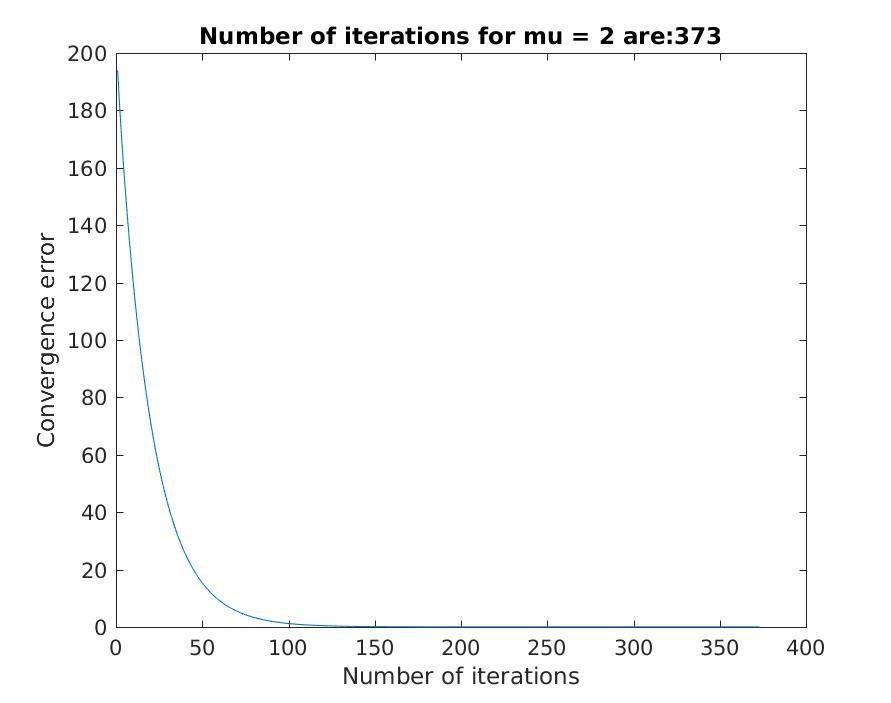
\includegraphics[width=0.5\linewidth]{richardson_2}
\caption{Convergence Plot for $\mu = 2$. Number of iterations are 373}
\end{figure}

\begin{figure}[H]
\centering
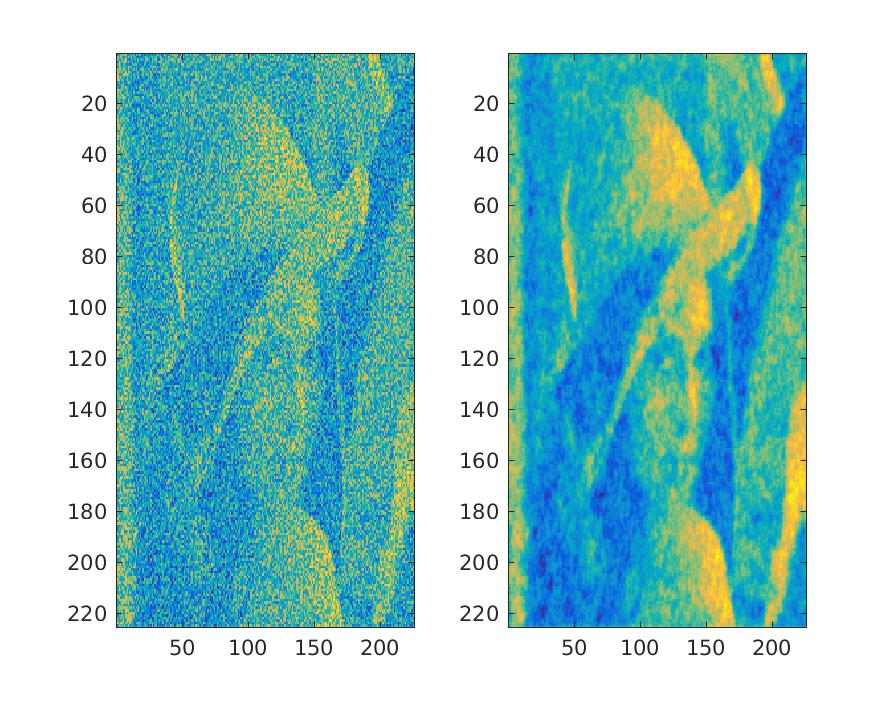
\includegraphics[width=0.5\linewidth]{richardson_denoised_2.jpg}
\caption{denoised image for $\mu = 2$}
\end{figure}


\begin{figure}[H]
\centering
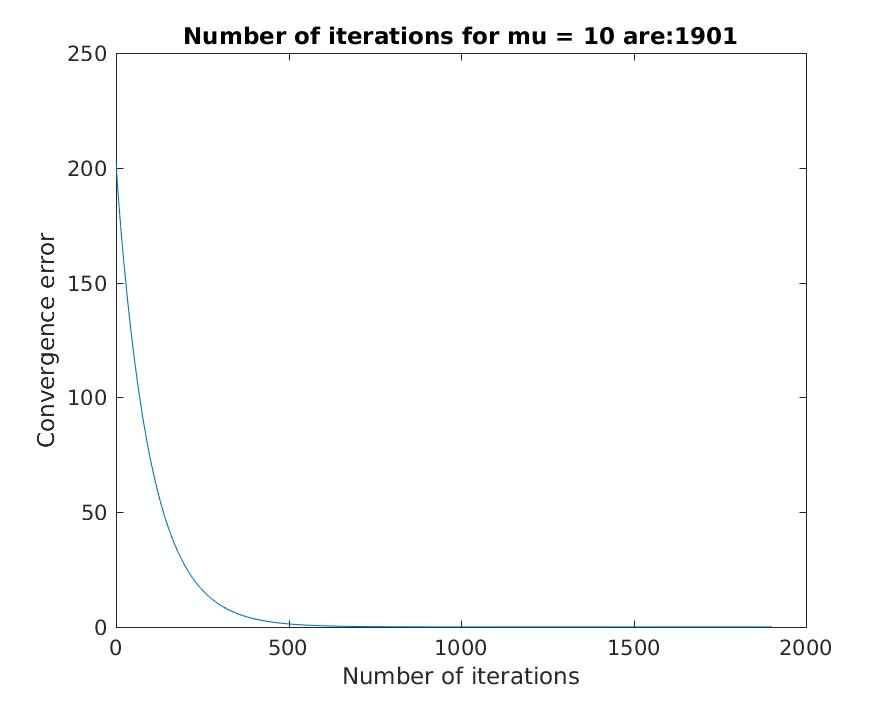
\includegraphics[width=0.5\linewidth]{richardson_10}
\caption{Convergence Plot for $\mu = 10$. Number of iterations are 1901}
\end{figure}

\begin{figure}[H]
\centering
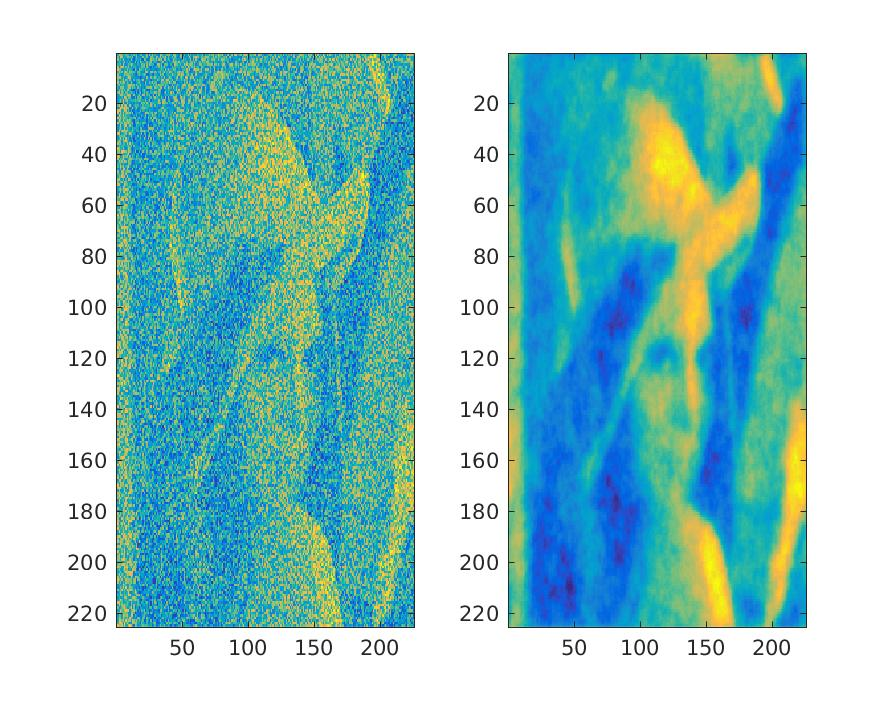
\includegraphics[width=0.5\linewidth]{richardson_denoised_10.jpg}
\caption{denoised image for $\mu = 10$}
\end{figure}


\subsection{Conjgrad}
d.)

\begin{figure}[H]
\centering
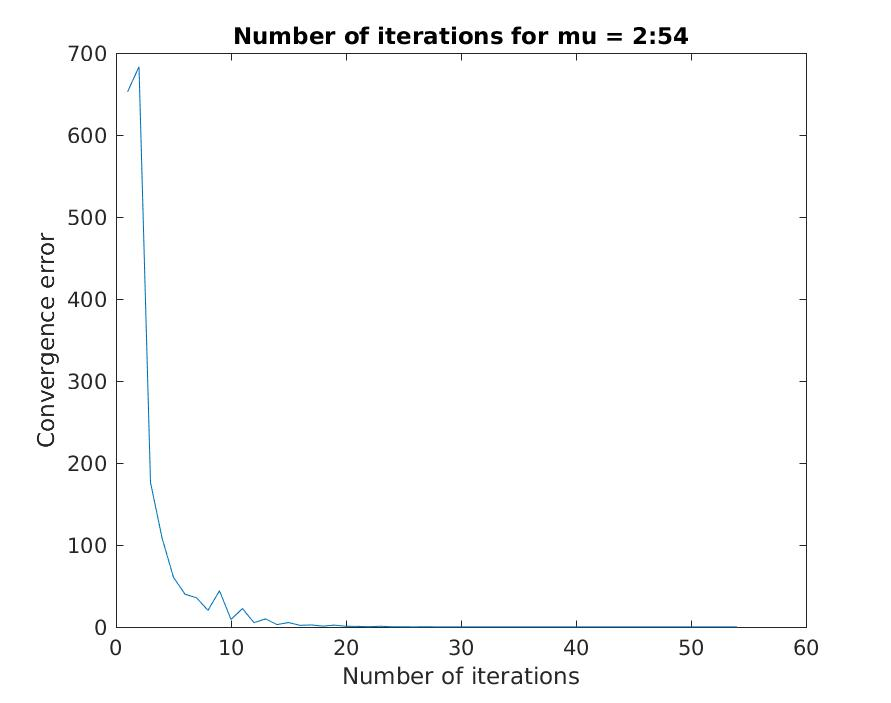
\includegraphics[width=0.5\linewidth]{conjgrad_2}
\caption{Convergence Plot for $\mu = 2$. Number of iterations are 54}
\end{figure}

\begin{figure}[H]
\centering
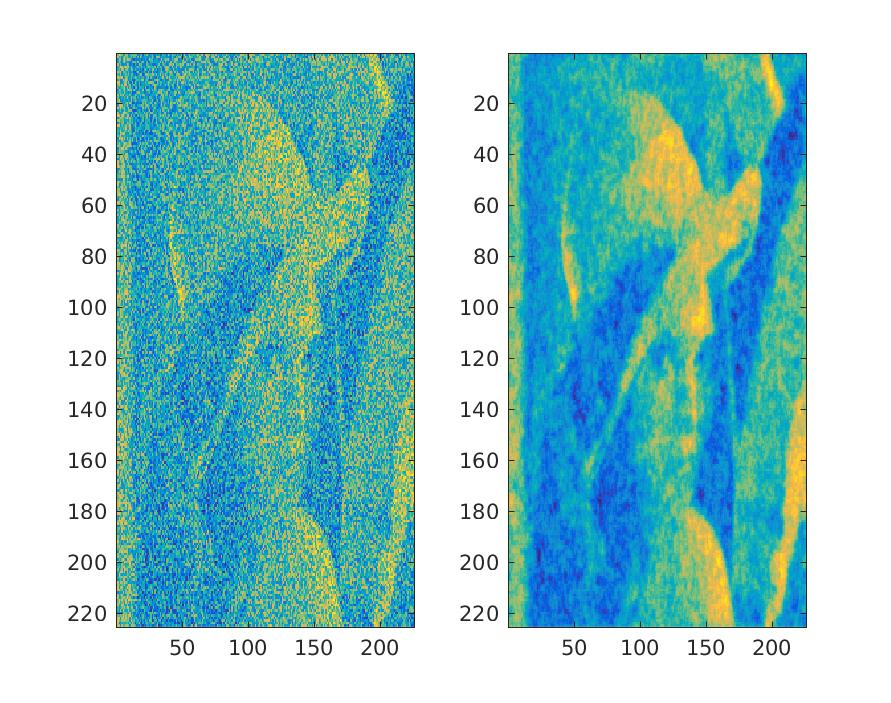
\includegraphics[width=0.5\linewidth]{conjgrad_denoised_2.jpg}
\caption{denoised image for $\mu = 2$}
\end{figure}


\begin{figure}[H]
\centering
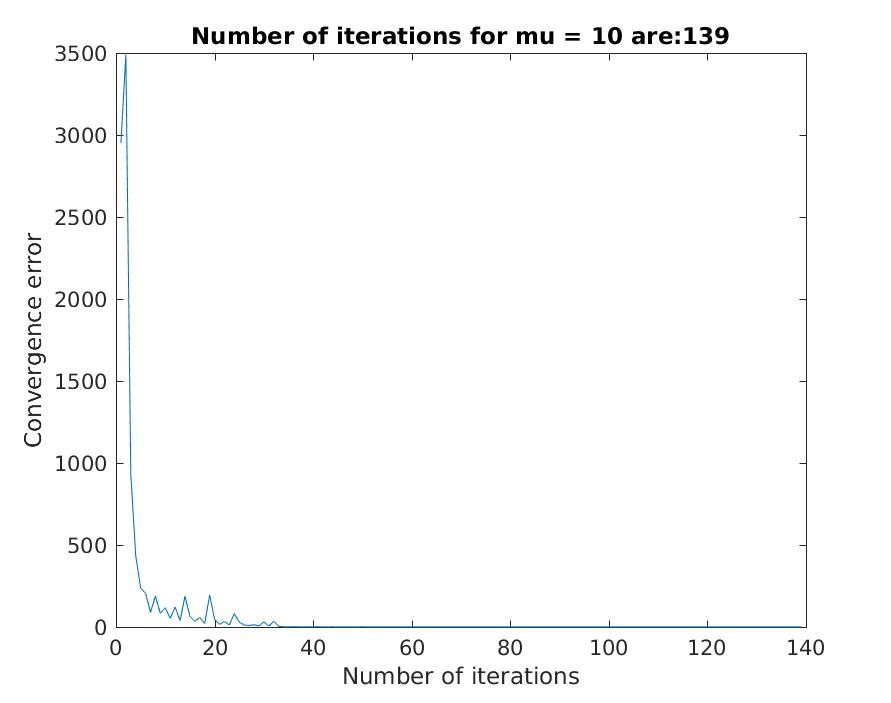
\includegraphics[width=0.5\linewidth]{conjgrad_10.jpg}
\caption{Convergence Plot for $\mu = 10$. Number of iterations are 139}
\end{figure}

\begin{figure}[H]
\centering
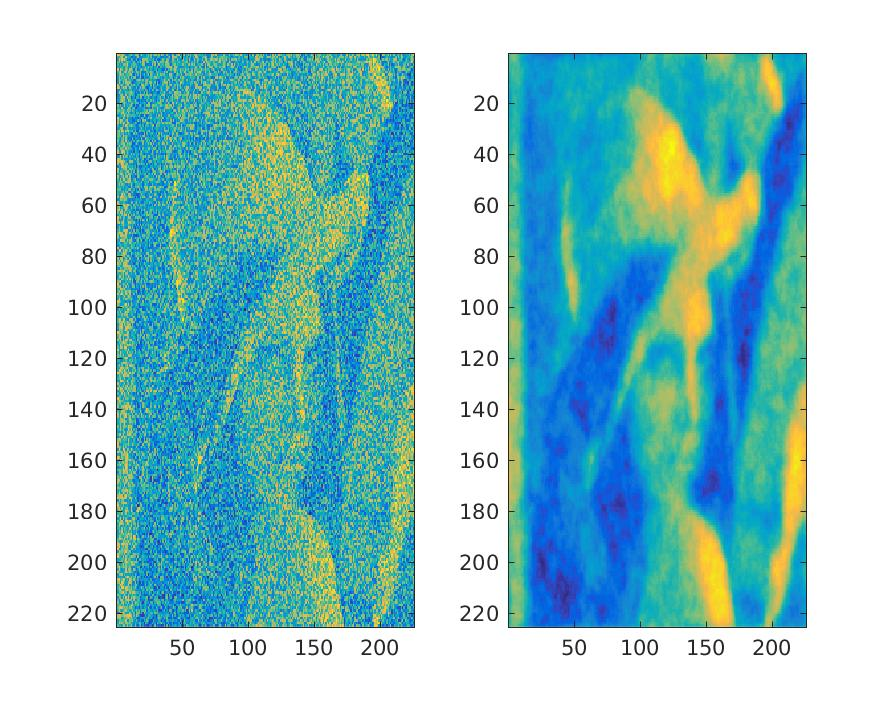
\includegraphics[width=0.5\linewidth]{conjgrad_denoised_10.jpg}
\caption{denoised image for $\mu = 10$}
\end{figure}

e.) It is observed that iteration counts increases both for Richardson iteration and conjugate gradient method.\\

\textbf{Stability Restriction}\\
According to the stability criterion, we can write out the taylor approximation of a convex function as, $f(y)\leq f(x) + (y-x)^T \nabla f(x) +\dfrac{M}{2}\|y-x\|^2$. \\

Now moving in a step size $\tau$ in the direction of the gradient, we can re-write the equation as
$$f(y- \tau \nabla f(x)) \leq f(x) - \tau \nabla f(x))^T \nabla f(x) +\dfrac{M \tau^2}{2}\| \nabla f(x)\|^2$$ \\

This is equal to $$f(y- \tau \nabla f(x)) \leq f(x) + \dfrac{M \tau^2 -2 \tau}{2}\| \nabla f(x)\|^2$$\\

 $$\dfrac{M \tau^2 -2 \tau}{2} < 0 \implies \tau < \dfrac{2}{M}$$\\

This means that the the convergance rate is always less than $\dfrac{M}{2}$. Applying this to our problem, we can factorize our problem as $$\frac{1}{2} \mu \|\nabla x\|^2 + \|x - b\|^2 $$. \\

This can be re-written as $\frac{1}{2} \mu x^T \nabla^T \nabla x + x^Tx -2x^Tb + \|b\|^2$. This gives $$ \dfrac{\mu }{2} x^T(\nabla^T \nabla + I)x -2x^Tb + \|b\|^2$$\\

$ \dfrac{1}{2} x^T(\mu \nabla^T \nabla + \mu I)x -2x^Tb + \|b\|^2$ is a quadratic where $\nabla^T \nabla$ is the laplacian and $\mu \nabla^T \nabla + \mu I$ is the hessian matrix. Let $\lambda $ be the largest eigenvalue of this hessian. That would be the largest curvature of the quadratic and convergence is defined when $$\tau < \dfrac{2}{\lambda}$$

\textbf{By this, we can see that $\tau$ depends inversely on $\mu$ as $\dfrac{2}{largest\ \ eigenvalue\ \ of(\mu \nabla^T \nabla + \mu I)}$ Hence as $\mu$ increases, $\tau$ decreases and hence results in slower convergence.}


\subsection{L2Denoise}
f.)
\begin{figure}[H]
\centering
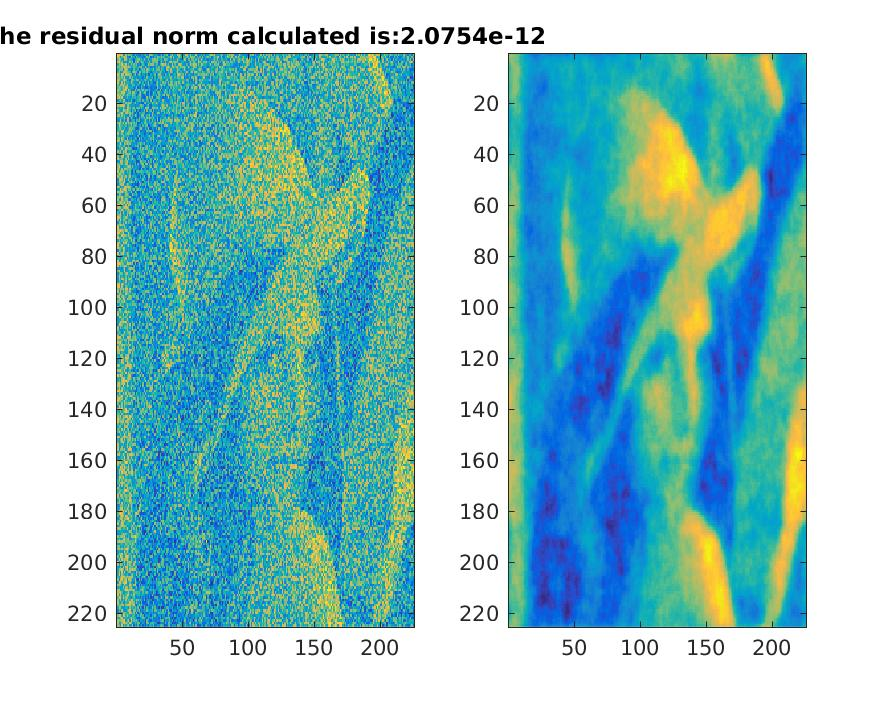
\includegraphics[width=0.5\linewidth]{l2denoise.jpg}
\caption{denoised image with $norm = e^{-12}$}
\end{figure}




\section*{Question 2}

\begin{figure}[H]
\centering
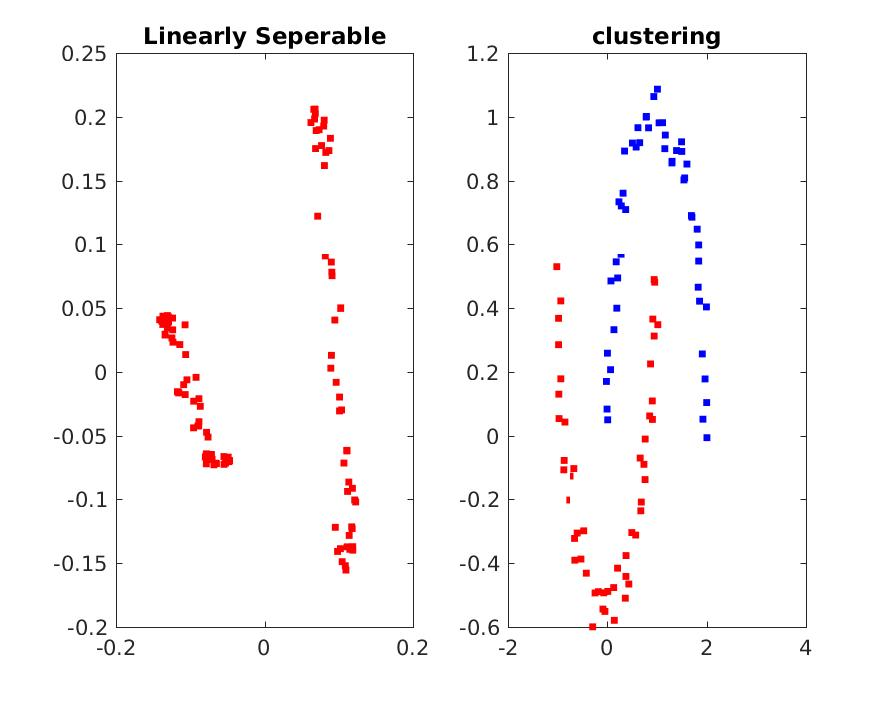
\includegraphics[width=1\linewidth]{1e2_points_clustering.jpg}
\caption{linear seperation and clustering for 100 points}
\end{figure}










\section*{Question 3}


\begin{figure}[H]
\centering
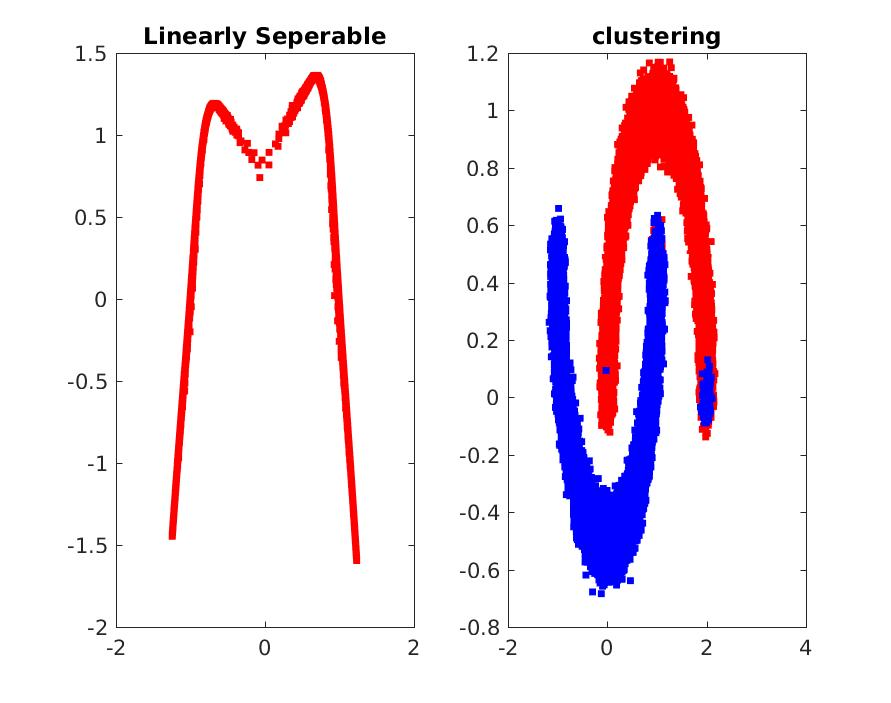
\includegraphics[width=1\linewidth]{1e5_points_clustering.jpg}
\caption{linear seperation and clustering for 100,000 points}
\end{figure}



% \end{equation}

% \begin{figure}[H]
% \centering
% \includegraphics[width=.75\linewidth]{xkcd_image}
% \end{figure}

%%%%%%%%%%%%%%%%%%
%                Text output
%%%%%%%%%%%%%%%%%%
% \newpage % Put the console output on a fresh page to make it look all pretty.
% \section*{Output from hmwk3.m, Question 2}
% % The verbatim environment is good for reproducing text without having latex try to format it for you.
% \begin{verbatim}

% The minimum error for Q2 is 8.8171e-07

% iscorrect =

%   logical

%    1


% \end{verbatim}


% \section*{Output from hmwk2.m, Question 3}
% % The verbatim environment is good for reproducing text without having latex try to format it for you.
% \begin{verbatim}


% The minimum error for Q3 is 3.6196e-08

% iscorrect =

%   logical

%    1

% \end{verbatim}


%  Now we're done.
\end{document}
